\chapter{绪论}\label{chapter_introduction}

本章首先介绍本文的研究背景,引出课题的动机、目的以及研究意义,
接着介绍现有解决方案概况,
最后介绍本文的主要工作以及后续章节的内容安排。

\section{研究背景}

随着工业的发展,各种零件的需求量大幅度增长,但是在零件的自动化生产中,由于加工设备或环境等因素,不可避免的导致零件缺陷的出现。常见的零件缺陷有裂纹、起皮、拉线、划痕、凹坑、凸起、斑点、腐蚀等,严重的甚至会出现偏芯、气孔。这些缺陷零件一旦流出,不仅可能在高级的设备组装时被发现、召回和索赔,更有可能在设备实际使用中造成故障,甚至引发事故。因此,传统零件加工中通常雇佣大量工人使用肉眼检测缺陷,这种方法往往浪费大量人力、财力,仍然难以取得较好效果。如图
\ref{fig:changguilingjian}中列举了几种常见的金属零件,金属零件大部分呈环状,而缺陷往往就出现在这些环形区域的表面。
\begin{figure}[htbp]
\centering
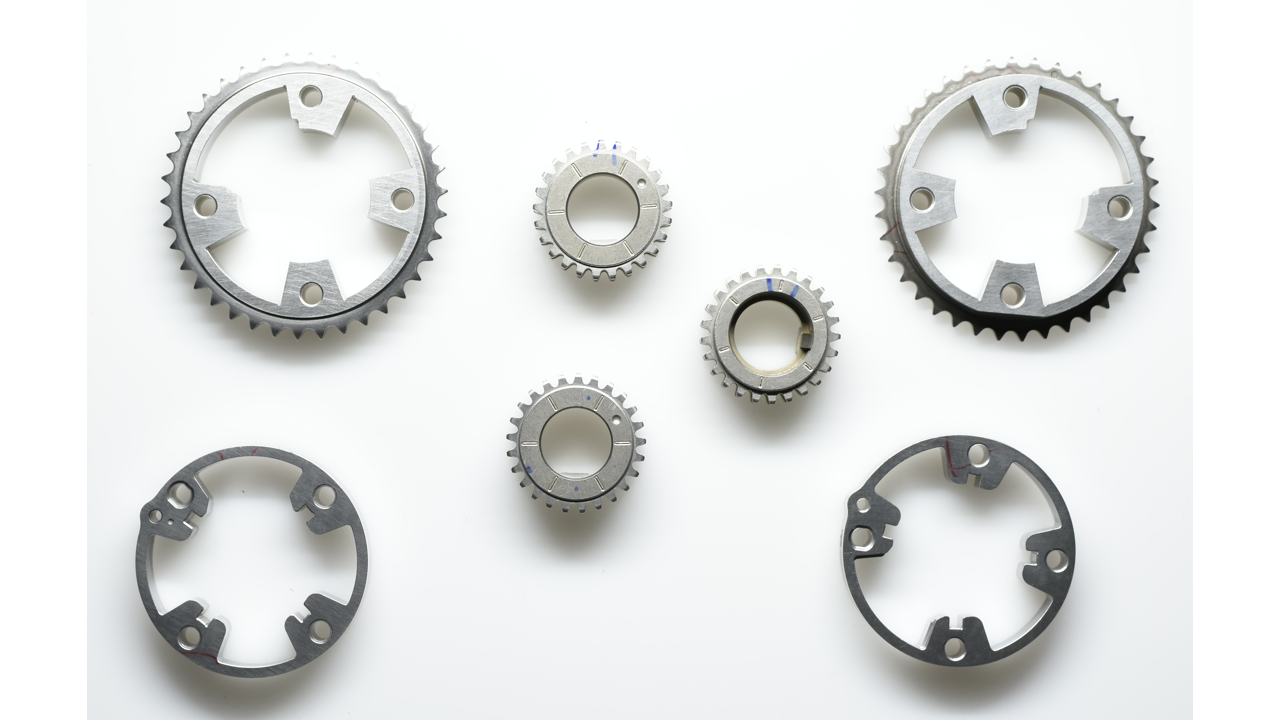
\includegraphics[width=0.8\textwidth]{figures/changguilingjian.png}\\
\caption{常规金属零件图}\label{fig:changguilingjian}
\end{figure}

在计算机视觉领域,缺陷检测是目标检测的一个重要应用。目标检测是通过计算机算法模拟人眼获取图片中感兴趣目标的过程,这一过程对于人类来说是一种本能,如同呼吸喝水一样简单,
但是对于计算机来说,
图片数据仅仅是$[0-255]$范围内的数字,
它很难理解这些信息所代表的含义,更分不清楚其中有什么物体以及这些物体所在的位置。
因此,对于计算机来讲,目标检测无疑是一项非常艰巨的任务。

传统的目标检测一般由获取原始图像、数据预处理、特征提取、训练分类器、使用分类器得到检测结果这几个步骤构成。其中特征提取是提取人工设计的特征,如梯度直方图\cite{dalal2005histograms}(Histogram of Oriented Gradients,简称 HOG)特征、
局部二值化\cite{ojala2000gray}(Local Binary Patterns,简称 LBP)特征
、
灰度共生矩阵\cite{haralick1973textural}(Gray-level Co-occurrence Matrix,简称GLCM)特征、
Oriented FAST and Rotated BRIEF\cite{rublee2011orb}(简称 ORB)特征等等。
传统分类模型主要包括决策树、支持向量机、逻辑斯特回归等。
这些分类器在某些问题上卓有成效,但是由于数据质量、特征设计、模型描述能力等因素限制,泛化能力有限,难以达到实际应用需要。
随着深度学习的发展,这类方法在分类和目标检测领域取得了非常好的效果,然而,这类模型要想取得较好结果,往往要求用海量数据对模型训练,并且动辄拥有上百层的网络结构,这种复杂的结构使得模型提取出的分类特征过于抽象,往往对于小目标难以取得较好效果,而在零件缺陷检测问题中,许多零件本身就不大,零件的缺陷则更小,深度学习往往难以奏效。

针对传统算法和深度学习算法的各自缺点,本文首先设计了提取零件法线图的方法,接着将法线图作为传统缺陷检测算法和深度学习缺陷检测算法的输入,进行缺陷检测,取得了理想的效果。

\section{现有工作概述}

在法线获取领域中,市面上最早出现的系统是
2013年Vizoo公司推出的Vizoo3D xTex,这是一款以相机为核心的表面信息提取系统,它通过相机对物体进行拍摄,然后使用一系列算法计算出材质的法线、
漫反射、高光以及透明度信息,是目前比较成熟的扫描系统,
但是该系统计算得到的法线并不精确。
目前国内也有
类似的系统,如厦门启尚科技研发的FSM 3D高清面料扫描仪,这款扫描仪小巧快
速,但是能够扫描的物体有限,并不能获取零件表面法线。

在目标检测领域,
传统的目标检测一般由获取原始图像、数据预处理、特征提取、训练分类器、使用分类器得到检测结果这几个步骤构成,如图\ref{chuantongjiancebuzhou}所示。
\begin{figure}[htbp]
\centering
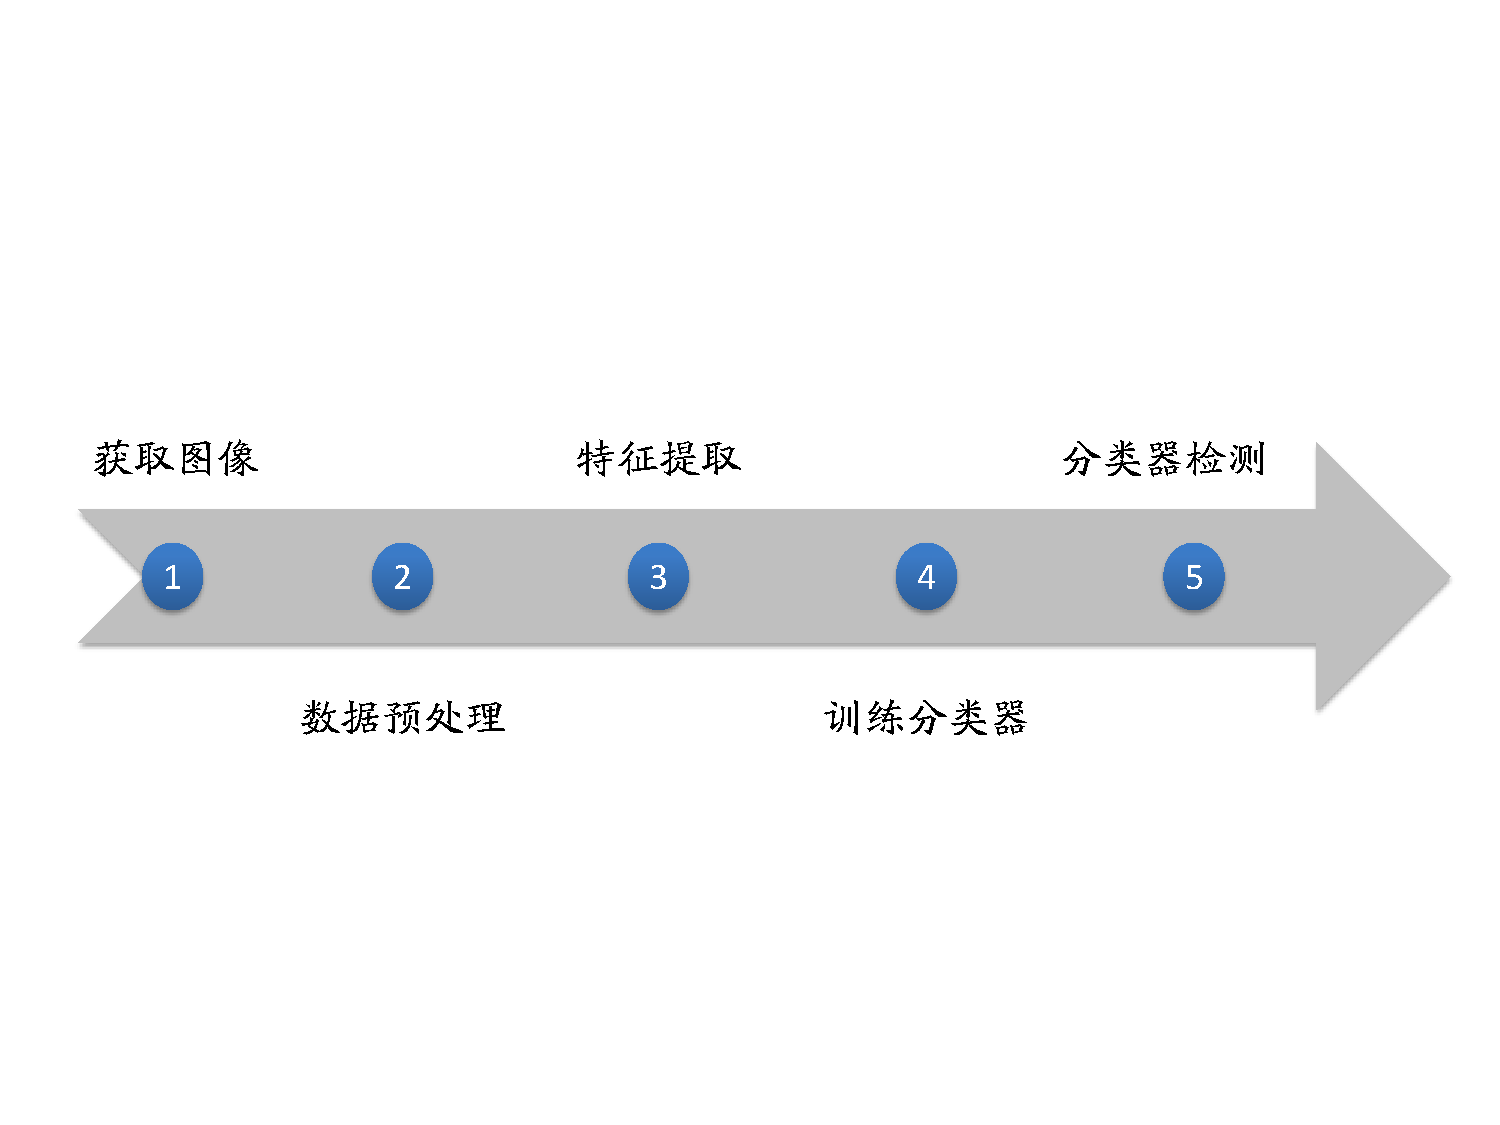
\includegraphics[width=1.0\linewidth]{figures/chuantongjiance.pdf}\\
\caption{传统方法缺陷检测步骤}\label{chuantongjiancebuzhou}
\end{figure}
在特征提取阶段,常用的特征有LBP特征、HOG特征、CLCM特征、哈尔\cite{viola2001rapid}(Haar-like)特征等等。
在分类器训练和检测阶段,一般采用不同尺寸的滑动窗口选择候选窗口用于训练和分类。
在分类器的选择中,
大多使用支持向量机\cite{hearst1998support}(Support Vector Machine,简称SVM)等传统的分类器模型。
其中,多尺度形变部件模型\cite{felzenszwalb2010object}(Deformable Part Mode,简称DPM)曾连续获得VOC(Visual Object Class)2007到2009的检测冠军,效果较好。
该算法将物体看成多个部件构成的整体,用部件之间的关系来描述物体,它继承了HOG和SVM各自的优点,但是模型的复杂度过高,检测速度不理想。

总的来说,传统的目标检测算法主要存在三个问题:
一是基于滑动窗口的窗口选择策略没有针对性,导致窗口冗余,时间复杂度过高;二是手工设计的特征往往对图片多样性的变化缺乏鲁棒性,并且在特征设计和选择阶段异常的复杂繁琐;三是分类模型往往泛化能力较弱。

自卷积神经网络\cite{lecun1998gradient}(Convolutional Neural Network, 简称 CNN)出现以来,产生了许多成熟的分类框架,其中最具代表性的有LeNet\cite{lecun1998gradient}、
AlexNet\cite{krizhevsky2012imagenet}、
VGG\cite{simonyan2014very}、
GoogleNet\cite{szegedy2015going}、
ResNet\cite{he2016deep}等。
LeNet是CNN的开山之作,被用于手写数字的识别,其后Alex Krizhevsky 提出了AlexNet,一举获得了2012年的ILSVRC比赛冠军
,该模型无论是速度还是精度都将第二名远远甩在身后。再之后的模型如VGG、GoogleNet不断加深网络结构,进一步提升了效果。但是随着模型的不断加深,模型极易出现梯度消失和梯度爆炸的问题,导致模型难以收敛,Kaiming He研究了这一问题,提出了ResNet模型,该模型增加了从低层到高层的“高速通道”,有效缓解了这一问题。

基于深度学习的目标检测算法大都构建于这些基础的分类框架之上,这些算法包括两大类:
一类以R-CNN\cite{girshick2014rich}
为代表,
包括R-CNN\cite{girshick2014rich}、Fast R-CNN\cite{girshick2015fast}、
Faster R-CNN\cite{ren2015faster}、Mask R-CMM\cite{he2017mask}、
RFCN\cite{dai2016r}等,
该类方法包含两个过程,首先是利用候选区域推荐(Region Proposal,简称RP)选出候选窗口,
接着是使用深度学习分类模型将这些候选分为目标窗口或背景窗口,
该类方法的主要问题是候选区域推荐复杂度高,所需时间久,很难达到实时;
另一类是以YOLO\cite{redmon2016you}为代表的基于深度学习的回归方法,这类算法包括YOLO、YOLO v2\cite{redmon2016yolo9000}、YOLO v3\cite{yolov3}、
Single Shot MultiBox Detector\cite{liu2016ssd}(SSD)、Deconvolutional Single Shot Detector\cite{fu2017dssd}(DSSD)等,
它们无需候选区域推荐,而是改用网格的方式将图像划分成不同的窗口,然后使用卷积优化的方法加速计算,该类算法简化了目标检测流程,提升了检测速度,但算法抛弃了候选区域推荐,导致模型学习到的物体特征并不精细,效果没有第一类方法好。此外,这些目标检测算法往往会产生许多互相重叠的候选窗口,需要使用非极大值抑制算法来确定最终目标窗口。
这些算法的主要有两个缺点:首先,深度网络模型的训练需要大量数据;最后,深度学习模型对于小目标物体检测效果不理想。

\section{本文工作和组织结构}

本节首先概述本文的主要工作和创新,接着介绍本文章节结构,并对各个章节内容做简要陈述。

\subsection{本文工作}

针对传统算法和深度学习算法各自的缺点,
本文首先从硬件设计和算法设计两个角度出发,
提出基于光线反射原理计算零件表面法线的方法,
接着将其作为传统缺陷检测算法的输入,
取得了理想的效果。
我们还将法线图应用到深度学习算法中,对比和分析了二者的结果。
本文的主要工作和创新有:
\begin{enumerate}

\item 本文提出了一种零件表面法线提取算法,包括硬件设计与算法设计两部分内容。
算法使用不同方向光源下拍摄得到的零件照片作为输入,基于光线的反射原理计算零件表面法线。
首先,我们设计了一套硬件设备,该设备包括遮光模块、平台模块、灯光模块、拍照模块和控制模块五大模块,
这些模块将相机、步进电机、LED灯带、滑轨、偏光镜和滤光膜等不同硬件组合成一个整体,
可以捕获不同方向光源下的零件照片。
接着我们将设备得到的零件照片作为法线计算算法的输入,提取零件法线。
为了优化照片的质量,提高零件法线的精度,
在实施法线计算算法之前,
本文首先对相机进行校正,
并对方向光源产生的光线损失进行光线补偿。
校正算法包括白平衡校正、色彩校正、畸变校正。
补偿算法首先预存储一套补偿数据,接着利用它对新的照片进行补偿。
值得一提的是,我们的法线提取算法不仅可以用来获取零件表面法线,还可以用来获取其他材质的表面法线。

\item 本文将法线图作为缺陷检测算法的输入,
研究了该背景下的最优特征组合及基于Adaboost方法的强分类器组合,
对传统的缺陷检测算法进行了改进,
并在进行了充分的实验验证。
本文首先使用传统检测算法进行检测,算法包括数据预处理、特征提取、设计和训练分类器以及用分类器进行检测等步骤。
在数据预处理阶段,
我们首先使用零件主表面提取算法滤除照片中的无关背景,
接着使用数据增强的方法扩大数据规模。
在特征提取阶段,我们分别提取了Haar-like特征、图像梯度特征、LBP特征、GLCM特征、HOG特征等不同的图像特征,并分析了不同特征的分类效果,根据分类效果对特征进行组合,从而得到一组最优特征组合。
在分类器分类阶段,
由于缺陷零件较少,
导致样本分布不平衡,
我们使用随机抽样的方法将数据集划分为不同的子数据集,
使每个子数据集拥有平衡的样本分布。
在训练阶段,我们使用支持向量机作为基分类器,对于每个子数据集,我们训练多个不同的基分类器,并利用Adaboost的方法将其组合成一个强分类器,
最终每个子数据集得到一个强分类器。
在检测阶段,
我们将这些强分类器组合成级联检测器,进行缺陷检测。

\item 本文将法线图作为深度学习模型的输入,
实验了基于深度学习的缺陷检测算法。
本文首先使用滑动窗口的方式将法线图分割成不同的窗口,
接着使用分类模型对这些窗口做分类。
在准备数据阶段,我们使用与传统算法中相似的预处理方法对数据进行处理。
在模型设计阶段,我们针对零件缺陷检测问题调整和优化了模型。
在模型训练和检测阶段,我们同样将数据集划分为不同的子数据集,
每个子数据集训练一个模型,
并利用级联的方式将它们组成一个级联检测器。
最后本文还将深度学习模型的检测结果与传统检测方法的结果进行了对比,分析了二者各自的优缺点及原因。

\end{enumerate}
\subsection{本文组织结构}

本文分为绪论、表面法线提取、基于传统算法的缺陷检测、基于深度学习的缺陷检测、总结和展望五个章节。本节所在章节为绪论,本章首先介绍本文工作的动机、目的和意义,概述本文课题的研究背景,接着介绍相关工作各自优缺点,进一步引出本文工作,并对本文工作作出简要概括,提出本文的主要创新,最后陈述本文章节结构和各章节内容。

第二章为零件表面法线提取,该章首先介绍为提取法线设计的独特硬件设备,接着展开描述以该设备获取数据为输入的表面法线提取算法,算法中包括对拍摄照片的校正算法如白平衡校正、色彩校正、畸变校正,以及对光线的补偿算法。

第三章为基于传统算法的缺陷检测,
该章依次介绍了
针对缺陷检测进行数据预处理和数据增强的方法、
提取法线图不同特征以及组合这些特征的方法、
设计和训练分类模型的方法
以及如何使用训练好的模型做检测的方法。在该章最后,给出了我们的实验结果以及分析,这些结果不仅包括使用法线图的特征作为输入训练和分类的结果,还包括使用常规零件照片的特征作为输入训练和分类的结果。

第四章为基于深度学习的缺陷检测,该章首先介绍卷积神经网络的基本结构,
接着详述本文使用的网络模型,并给出数据预处理和数据增强的方法,
接着介绍如何用得到的数据使用模型进行训练和检测,最后给出实验结果,并将其与第三章的结果进行对比和分析。

第五章为总结和展望,该章首先对本文的工作做出总结,接着提出本文工作中存在的不足以及可以改进之处。